\chapter{Introduction}
\minitoc
\label{Cap:Int}
%%%%%%%%%%%%%%%%%%%%%%%%%%%%%%%%%%%%%%%%%%%%%%%%%%
% 
\section{Standard Model}
\label{Cap:Int:SM}
The Standard Model of Particles (SM) is a unified quantum field theory of the electroweak interaction and Quantum Chromodynamics (QCD). It describes fundamental entities known as quantum fields, which represent 17 elementary particles, each accompanied by its respective antiparticle.

The elementary particles are divided in two main blocks: 
\begin{itemize}
    \item The fermions, which are commonly know as the matter particles (or antimatter particles). These are half-integer spin particles and are divided in two categories, quarks and leptons. 
    \item Bosons are carriers of weak, strong, and electromagnetic fundamental interactions. The spin of the bosons is always an integer. It also includes the Higgs field, whose interactions with other particles cause those particles to acquire mass.
\end{itemize}

The agreement between the SM predictions and particle physics experiments provides a high confidence in this model. However, it is not complete; there are phenomena that are not described by it, such as dark mater and neutrino oscillations.

\begin{figure}[!htb]
\centering
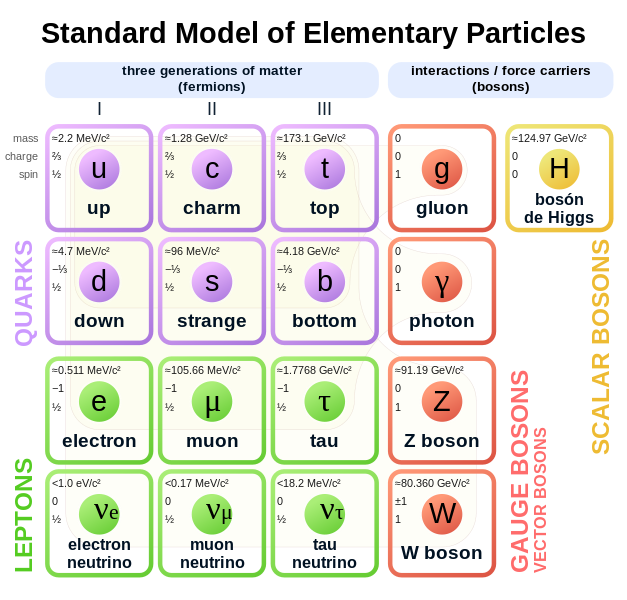
\includegraphics[scale=0.5]{Figures/Chapter1/Standard_Model_of_Elementary_Particles.png}

        \caption{In the figure is shown a pictorial summary of the  17 particles of the SM. Something that should be considered is that there are other 17 that correspond to the antiparticle of each particle. Figure from \cite{SM_Table}.} 
\label{fig:SM}
\end{figure}
 
\subsection{Bosons}
In the SM, the elementary particles interact through the gauge bosons, which act as carriers for the fundamental forces of weak, strong, and electromagnetic interactions. The Higgs boson plays a crucial role in the Higgs mechanism, whereby particles gain mass through their interaction with this boson. Additionally, there is a hypothetical boson called graviton; this particle should be the carrier of the gravitational force, it has not been observed yet. Bosons have integer values for spin.  

\subsubsection{The electromagnetic force}
Described by quantum electrodynamics, the electromagnetic force is transmitted by photons, which interact exclusively with charged spin 1/2 particles. The mass of the photons is 0. This force is capable of acting over long distances. This is responsible for the effects of electromagnetic force being observable on a macroscopic scale, and it finds numerous practical applications.

\subsubsection{Strong Force}
It is carried by the gluons, which are responsible for binding quarks and generating hadrons. This force is also responsible for the binding of the neutrons and protons in the interior of the atomic nucleus. Interactions mediated by the strong force are modeled by quantum chromodynamics (QCD). Here, the charge is represented as "color", which is carried only by quarks.

In QCD, there are three color charges (red, blue, and green). The quarks have one charge color each;  the gluons have two colors -color and anticolor-. In strong interactions, the color of the quarks may change, but as is the case with the electric charge, color is always conserved. Unlike photons, the gluons are capable of interacting with other gluons, which makes it more complicated to consider all the interactions that occur between them; this property is known as self-coupling. The color charge cannot be observed directly in nature due to a property know as \textit{color confinement}; therefore the quarks are not observed isolated. 

The strong force increases as the distance between the quarks increases. For processes in which the rupture of a nucleon is observed by the scattering of other particles, internally the gluon produces a quark-antiquark pair from the vacuum using the energy acquired from the incoming particle to create other hadron, this process is called \textit{hadronization}.

 

\subsubsection{The weak force}
It is carried by the bosons $W^\pm$ and $Z$, which are responsible for various particles decays and some scattering processes. This is a short-range force, due to the large mass of the W and Z bosons. These couple with the quantum property called \textit{flavor}. All elementary fermions may interact by this interaction; in the case of neutrinos, it is the only known way that this particle interacts.

There are two types of weak force interaction, the charged current (CC) interaction and the neutral current (NC) interaction. The CC interactions occur when particles interact by the $W^\pm$ boson. The $W^\pm$ boson and can therefore also interact with photons. The W boson changes the interacting particles to the weak isospin doublet partner. 

The weak (lepton) isospin doublets:
$\begin{pmatrix}
    \nu_e \\
    e^-
\end{pmatrix}$, 
$\begin{pmatrix}
    \nu_\mu \\
    \mu^-
\end{pmatrix}$, 
$\begin{pmatrix}
    \nu_\tau \\
    \tau^-
\end{pmatrix}$


Tree doublets are called leptons; these are described later. The flavor of the leptons is always conserved in the CC interactions. 

The quark isospin doublets:

$\begin{pmatrix}
    u \\
    d
\end{pmatrix}$, 
$\begin{pmatrix}
    c \\
    s
\end{pmatrix}$, 
$\begin{pmatrix}
    t \\
    b
\end{pmatrix}$

In the case of the quark sector, the six members can interact with any quark. It is because the mass eigenstates are different from their mass eigenstates. The CKM matrix (Cabibbo-Kobayashi-Maskawa) describes how these can be mixed. 

 NC interactions are mediated by the Z boson. These interactions do not change the identity of the particles. Some examples of this kind of interactions are the neutrino-nucleon scattering (NC $\nu$ -N interaction) and the neutrino-electron scattering (NC $\nu$ -e interaction). 



\subsection{Fermions}
These are the blocks of matter; 12 of the 17 fundamental particles are fermions, these are defined as particles with half-integer spin. These are divided into quarks and leptons. 

\textbf{Quarks.}
The quarks are described by QCD, a gauge theory based on SU(3) symmetry.  

\textbf{Leptons.}
In the SM, there are six different leptons, along with their respective antiparticles. These are divided into 3 groups called generations, these can be represented by doublets: 

$\begin{pmatrix}
    \nu_e \\
    e^-
\end{pmatrix}$, 
$\begin{pmatrix}
    \nu_\mu \\
    \mu^-
\end{pmatrix}$, 
$\begin{pmatrix}
    \nu_\tau \\
    \tau^-
\end{pmatrix}$

The electron $e^-$, the muon $\mu^-$ and the tau $\tau^-$ are electrically charged leptons; with a charge $-e$, where $e$ is the magnitude of the charge of the electron, these leptons interact by weak electromagnetic forces and weak forces. 

The $\nu_e$, $\nu_\mu$ and $\nu_\tau$ are electrical neutral leptons, that only interact by weak force. These leptons are known as neutrinos and depending the generation these are called electron-neutrino ($\nu_e$), muon-neutrino ($\nu_\mu$) or tau-neutrino ($\nu_\tau$). 

\section{Neutrinos}
The neutrinos are the most abundant massive particles in the universe of the SM. They are leptons with no electrical charge. The neutrinos only interact by the weak interaction, which means they do not interact very frequently. 

\subsection{A brief story of the neutrinos}
During the beginning of last century, nuclear physicists studied the radioactivity of different materials. During these studies, they identified mainly 3 types of nuclear decays: $\alpha$ -decay, $\beta$ -decay, and the $\gamma$ -decay. The energy of $\alpha$-decay and $\gamma$-decay is discrete and depends on the atomic nucleus that emits the radiation. The energy spectrum shows characteristic peaks for certain values of energy; in \textbf{Figure} \ref{fig:abgSpectrum} two examples of energy spectrum for alpha and gamma emissions are shown. On the other hand, $\beta$-decay processes produce continuum spectra; in \textbf{Figure} \ref{fig:abgSpectrum} an example of the $\beta$-decay energy spectrum is shown. The fact that the energy spectrum of the $\beta$-decay electron is a continuum indicates that a portion of the energy was lost or a violation of the energy conservation law.

\begin{figure}[!htb]
\centering
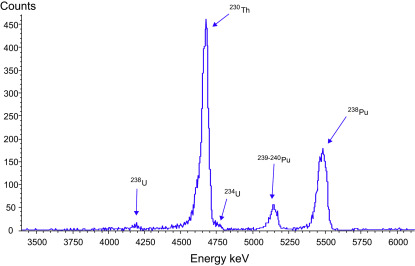
\includegraphics[scale=0.8]{Figures/Chapter1/alphaspectrum.jpg}
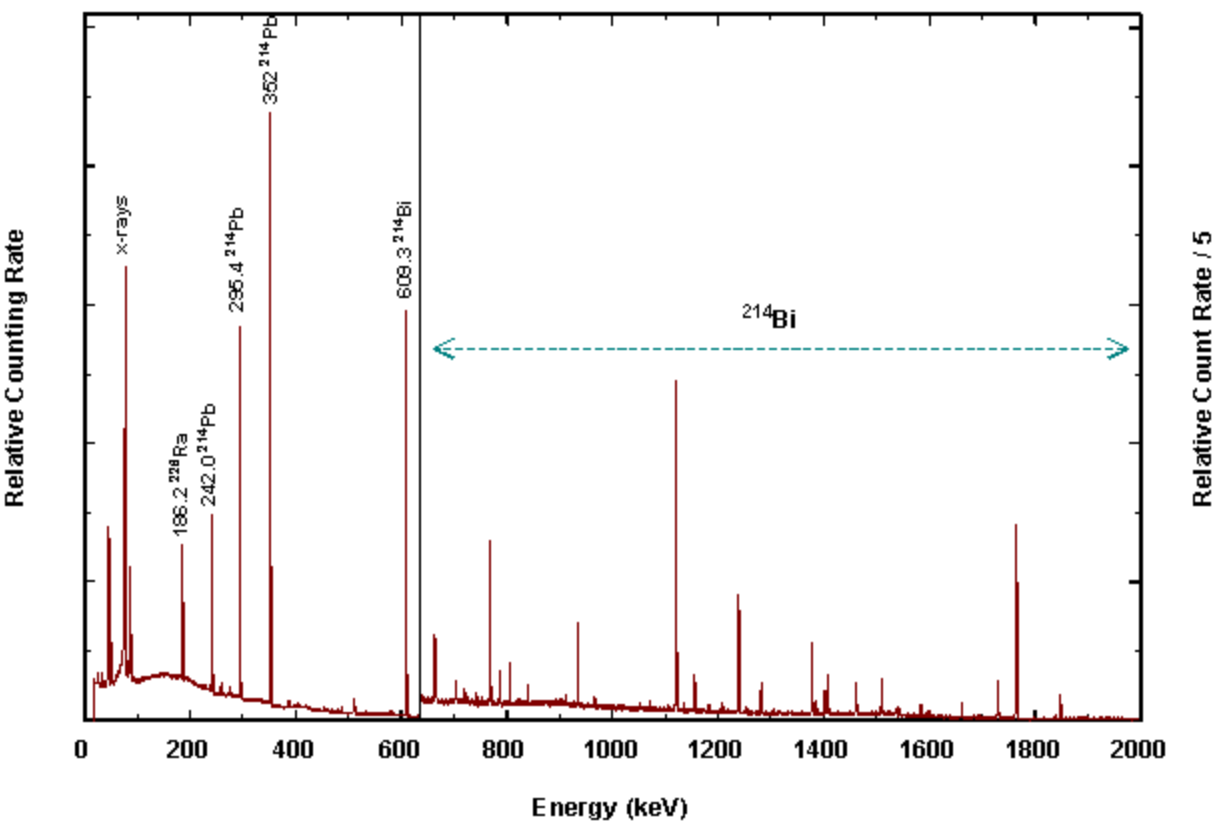
\includegraphics[scale=0.2]{Figures/Chapter1/radspec_gamma.png}
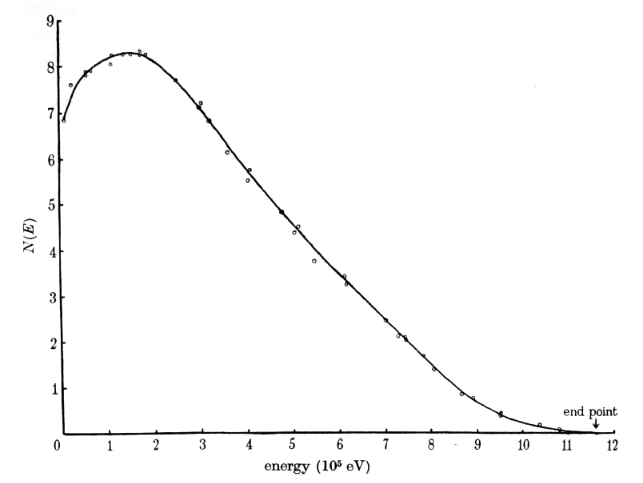
\includegraphics[scale=0.25]{Figures/Chapter1/Ra_betaSpec.png}

        \caption{Top plot, alpha spectrum of a mixture of radioactive materials measured by a gas detector\cite{alphaSpectrum}. Middle plot, gamma spectrum of Radium-226 from high purity germanium detector\cite{RaSpectrum_gamma}. Bottom plot, spectrum of energy of electron from beta decay in of Ra\cite{Ra_betaSpec}.} 
\label{fig:abgSpectrum}
\end{figure}

In 1930 Wolfgang Pauli \cite{NeutrinoHistory} proposed in a letter that the continuum spectra might be due to one more "invisible" light neutral particle, this should have spin 1/2 and obey the exclusion principle, he called this particle \textit{neutron}. In the letter Pauli explained that with this particle the electron would be able to take any momentum up to the maximum allowed limit, where the other particle has the residual momentum. In 1932 Chadwick discovered the neutron, which did not match Pauli's description. In 1933, Enrico Fermi adopted the name \textit{neutrino} for the particle proposed by Pauli; Fermi proposed a model where the neutrino should be a $^1/_2$ spin particle (a fermion). In 1953, neutrinos were observed by the experiment of Clyde Cowan and Frederick Reines \cite{CowanReinesdoi:10.1126/science.124.3212.103}\cite{ReinesCowanPhysRev.92.830}. In this experiment they measured the antineutrinos produced in the Savanna River Reactor in South Carolina. The products of the antineutrino interaction with a proton produced a neutron and a positron; the neutron is captured by Cd and emits two photons, while the positron interacts with an electron producing two photons. The light from the electrons is captured by photomultipliers.

\begin{figure}
    \centering
    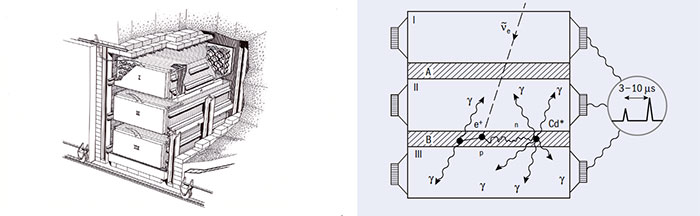
\includegraphics[scale=0.5]{Figures/Chapter1/RainesCowanExperiment.jpg}
    \caption{Scheme of the Raines and Cowan experiment. The figure shows how the neutrino interactions were detected by coincidence in time between the positron annihilation and the gammas produced by the decay of the neutron. Figure from \cite{ReinesCowanScheme}.}
    \label{fig:RainesCowanExperiment}
\end{figure}

\subsection{Neutrino Oscillation}
\label{Cap:Int:NuOscillation}

The SM initially describes neutrinos as massless particles that travel at a speed of light. However, the measurements of solar neutrinos and atmospheric neutrinos gave the first sign of physics beyond the SM.

In 1946, Pontecorvo proposed an experiment to detect $\Bar{\nu_e}$  through the reaction $^{37}$Cl + $\Bar{\nu_e} \rightarrow$ $e^- + ^{37}$Ar, followed by the counting of electron captures on $^{37}$Ar. In the 1950s, Davis et al. reported the results of the Homestake mines experiment in the United States \cite{PhysRev.86.976, PhysRev.97.766}. This experiment involved a tank filled with perchloroethylene located underground in a gold mine. The interactions of electron neutrinos with chlorine atoms produced electrons and $^{37}$Ar$^+$ ions, which were detected by counting electron captures. The reported flux was one third smaller than the flux of electron neutrinos predicted by the Bahcall solar model \cite{SolarModel}. One possible explanation for this discrepancy was the neutrino flavor oscillation, first proposed by Pontecorvo in 1957 \cite{Pontecorvo:1957cp}. Neutrino oscillation implies non-zero neutrino mass. Subsequent experiments such as the Sudbury Neutrino Observatory (SNO) and Kamiokande corroborated these results, revealing similar discrepancies with solar neutrino production, leading to what was known as the "Solar Neutrino Anomaly." Another discrepancy was observed in the measurement of atmospheric neutrinos by Super-Kamiokande, which showed a dependence of the muon neutrino flux on the zenith angle, known as the "Atmospheric Neutrino Anomaly.

Both anomalies are consistent with the neutrino oscillation model suggested by Pontecorvo. The complete description of the mechanism that gives mass and how it relates to neutrino flavors was developed by Ziro Maki, Masami Nakagawa, and Shoichi Sakata in the Pontecorvo-Maki-Nakagawa-Sakata (PMNS) matrix \cite{10.1143/PTP.28.870}. 

\subsection{Neutrino oscillations formalism}
It establishes that the neutrino flavor eigenstates ($\nu_1,\ \nu_2,\ \nu_3$) are related with the mass eigenstates as follow:

\begin{equation}
    \begin{split}
        \left|\nu_e\right> = a_1\left|\nu_1\right> + b_1\left|\nu_2\right> + c_1\left|\nu_3\right>\\
        \left|\nu_\mu\right> = a_2\left|\nu_1\right> + b_2\left|\nu_2\right> + c_2\left|\nu_3\right>\\
        \left|\nu_\tau\right> = a_3\left|\nu_1\right> + b_3\left|\nu_2\right> + c_3\left|\nu_3\right>
    \end{split}   
    \label{eq:MassEigenstatesSum}
\end{equation}

where a, b, and c are different coefficients. The coefficients can be written in a unitary matrix as follows:

\begin{equation}
    \begin{bmatrix}
        \nu_e \\ \nu_\mu \\ \nu_\tau
    \end{bmatrix}
    = 
    \begin{bmatrix}
        U_{e1} & U_{e2} & U_{e2}\\
        U_{\mu1} & U_{\mu2} & U_{\mu3}\\
        U_{\tau1} & U_{\tau2} & U_{\tau3}\\
    \end{bmatrix}
    \begin{bmatrix}
        \nu_1 \\ \nu_2 \\ \nu_3
    \end{bmatrix}.
\end{equation}

Condensing the equations from \ref{eq:MassEigenstatesSum} and the unitary matrix is obtained:

\begin{equation}
    \left|\nu_\alpha\right> = \sum_j U_{\alpha j}\left|\nu_j \right>
    \label{eq:CondensedPMNS}
\end{equation}

This is assuming that the neutrinos are Dirac particles, which means they are not their own antiparticles. This is known as the Pontecorvo-Maki-Nakasawa-Sakata (PMNS) matrix. The matrix can be expressed with only four parameters; the other five are related to the other four. The parameters are the mixing angles $\theta_{12}$, $\theta_{13}$ and $\theta$, and the $\delta_{CP}$. The mixing angles describe how the flavor eigenstates change by the rotation of the mass eigenstates. The $\delta_{CP}$ describes the strength of the CP violation. Re-writing the PMNS matrix with the four parameters we have:

\begin{equation}
    \begin{bmatrix}
        1 & 0 & 0\\
        0 & c_{23} & s_{23}\\
        0 & -s_{23} & c_{23}\\
    \end{bmatrix}
    \begin{bmatrix}
        c_{13} & 0 & s_{13}e^{i\delta_{CP}}\\
        0 & 1 & 0\\
        -s_{13}e^{i\delta_{CP}} & 0 & c_{13}\\
    \end{bmatrix}
    \begin{bmatrix}
        c_{12} & s_{12} & 0\\
        -s_{12} & c_{12} & 0\\
        0 & 0 & 1\\
    \end{bmatrix}
\end{equation}



where $s_{ij}$ and $c_{ij}$ are the $sin$ $\theta_{ij}$ and $cos$ $\theta_{ij}$, respectively. 

To calculate the probability of a neutrino oscillation to another flavor, the process starts  with the expression for a plane wave for a neutrino with mass eigenstate $j$ in free propagation: 
\begin{equation}
    \left| \nu_j (t)\right> = e^{-ip_j\cdot x_j}\left| \nu_j (0)\right>
\end{equation}

Assuming that it is an ultrarelativistic ($t\sim z$) neutrino and the $\Vec{x}$ components align to the $z$ direction, the phase for the neutrino mass eigenstates becomes 

\begin{equation}
    p_j\cdot x_j \approx \frac{m^2_j}{2E}z,
\end{equation}

This is obtained from $E_j = \sqrt{|\Vec{p}^2|+m^2_j}\approx |\Vec{p}| + \frac{m^2_j}{2|\Vec{p}|}$, assuming that the neutrino masses are small so that $E_j \sim |\Vec{p}_j|$. At the same time, given the small value of $m_j$ the mass eigenstates have approximately the same energy, $E=E_j$.

Then equation \ref{eq:CondensedPMNS} can be used to obtain the propagator for the eigenstate of the neutrino flavor $\alpha$ as a function of the distance where the neutrino was produced ($L$) as

\begin{equation}
    \left|\nu_\alpha (L)\right> = \sum_j U_{\alpha j}e^{-i\frac{m^2_j L}{2E}}\left|\nu_j \right>=\sum_\beta \left(\sum_j U_{\alpha j}e^{-i\frac{m^2_j L}{2E}}\right)\left|\nu_\beta \right>.
    \label{eq:NeutrinoPropagatorL}
\end{equation}

In this way, the equation is rewritten in the flavor basis $\beta$. Therefore, the probability of flavor oscillation as a function of $L$ is

\begin{equation}
    \begin{split}
        P_{\nu_\alpha\rightarrow\nu_\beta}(L) & =|\left<\nu_\beta | \nu_\alpha(L)\right>|^2 \\
        & = \sum_j\sum_k U_{\beta j} U^*_{\alpha j} U^*_{\beta k} U_{\alpha k} e^{-i\frac{(m^2_k - m^2_j)L}{2E}}
    \end{split}
\end{equation}

Defining $\Delta m^2_{kj}=m^2_k - m^2_j$, using the properties of $e^{ix}$ and using the properties of sines, the following expression is obtained:

\begin{equation}
    \begin{split}
        P_{\nu_\alpha\rightarrow\nu_\beta}(L) = & \delta_{\alpha\beta} - 4\sum_{j>k}\Re\left(U_{\beta j} U^*_{\alpha j} U^*_{\beta k} U_{\alpha k}\right) sin^2\left(\frac{\Delta m^2_{kj}L}{4E}\right) \\
        & \mp 2\sum_{j>k}\Im\left(U_{\beta j} U^*_{\alpha j} U^*_{\beta k} U_{\alpha k}\right) sin\left(\frac{\Delta m^2_{kj}L}{2E}\right)
    \end{split}
\end{equation}

where if $\delta_{CP}= 0$ or $\pi$, the imaginary term is zero. The sign for the imaginary term is negative, which corresponds to the neutrino oscillation probability, and the positive sign corresponds to antineutrino. 

The PMNS matrix originally comprises 4 parameters, but the calculation of oscillation probabilities introduces additional parameters: $L$, $E$, and $\Delta m^2_{kj}$. The values of $L$ and $E$ depend on where and how neutrinos are produced and measured. For the parameters $\Delta m^2_{jk}$, we have $\Delta m^2_{31} = \Delta m^2_{21} + \Delta m^2_{32}$, giving a total of 6 fundamental oscillation parameters, and $E$ that depends on the external conditions. The results of the experiments are used to determine the value of these free parameters.

In the argument of sine, the parameter that governs the behavior of the oscillation is the difference between the squared masses. In fact, it is not necessary to know the neutrino masses precisely. The results of the experiments report a small value of $|\Delta m^2_{21}|$ and a much larger difference for $|\Delta m^2_{31}|$ and $|\Delta m^2_{32}|$, being $|\Delta m^2_{31}| \cong |\Delta m^2_{32}|$. 

From the current experiments, the values of $|\Delta m^2_{21}|$, $|\Delta m^2_{31}|$, and $|\Delta m^2_{32}|$ are known, but not the sign of the squared mass differences. This raises new questions about the mass ordering. This is known as the neutrino mass hierarchy , giving two possibilities: the normal hierarchy where $m^2_1 < m^2_2 \ll m^2_3$, or the inverted hierarchy $m^2_2 > m^2_1 \gg m^2_3$.

\begin{figure}[!htb]
    \centering
    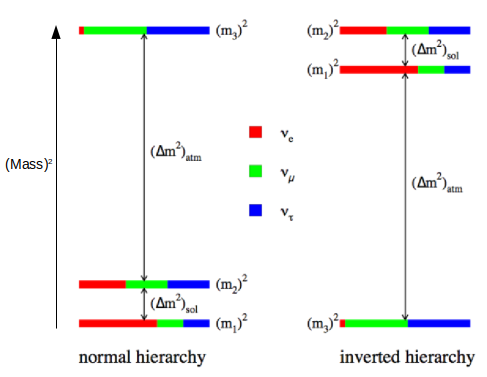
\includegraphics[scale=0.4]{Figures/Chapter1/MassHierarchy.png}
    \caption{Scheme illustrating the normal (left) and inverted (right) mass hierarchy. Figure from \cite{AaronThesis}.}
    \label{fig:Cap1:MassHierarchy}
\end{figure}

The value of $\theta_{12}$ and $\Delta m^2_{12}$ have been obtained from the results of the solar and reactor neutrino experiments, while the value of $\theta_{13}$ and has been obtained from the accelerator experiments and nuclear reactor neutrino experiments. For the parameter $\delta_{CP}$, the value can be estimated using the accelerator neutrino experiments, comparing the neutrino and antineutrino results. The most recent values of the oscillation parameters are shown in the \textbf{Table} \ref{tab:Cap1:OscillationParameters}.

\begin{table}[!htb]
    \centering
    \begin{tabular}{c|c}
        Parameter & Best fit \\ \hline
        $sin^2(\theta_{12})$ & 0.307 $\pm$ 0.013 \\ \hline
        $sin^2(\theta_{23})$ (IO) & $0.534^{+0.021}_{-0.024}$ \\ \hline
        $sin^2(\theta_{23})$ (NO) & $0.547^{+0.018}_{-0.024}$  \\ \hline
        $sin^2(\theta_{13})$ & (2.20 $\pm$ 0.07) $\times10^{−2}$ \\ \hline
        $\Delta m^2_{21}$ & (7.53 $\pm$ 0.018)$ \times\ 10^{-5}$ eV$^2$ \\ \hline
        $\Delta m^2_{32}$ (IO) &  (−2.519 $\pm$ 0.033)$\times10^{−3}$ eV$^2$ \\ \hline
        $\Delta m^2_{21}$ (NO) & (2.437 $\pm$ 0.033) $\times10^{−3}$ eV$^2$ \\ \hline
        $\delta_{CP}$ & 1.23$\pm$0.21 $\pi$ rad\\
    \end{tabular}
    \caption{Values of the oscillation parameters based in the experimental results assuming the normal ordering (NO) and the inverted ordering (IO). Table obtained from \cite{Workman:2022ynf}}.
    \label{tab:Cap1:OscillationParameters}
\end{table}

\section{Neutrino interactions}
\label{Cap:Int:NuInteractions}

The neutrinos interactions in the SM are mediated only by the boson Z$^0$ and W$^{\pm}$. In this section, the neutrino neutral current (NC) and charged current (CC) interactions are described.

\subsection{Neutral current interactions}
\label{Cap:Int:NuInteractions:NC}

Neutral current interactions are mediated by the Z$^0$ boson. The Weinberg-Salam (W-S) model, originally described in references \cite{PhysRevLett.19.1264} and \cite{Salam1959}, initially provides a good description of the elastic neutral current interactions.

Depending on the neutrino energy, it can interact via neutral current with electrons, nuclei, and nucleons.

\begin{figure}[!htb]
    \centering
    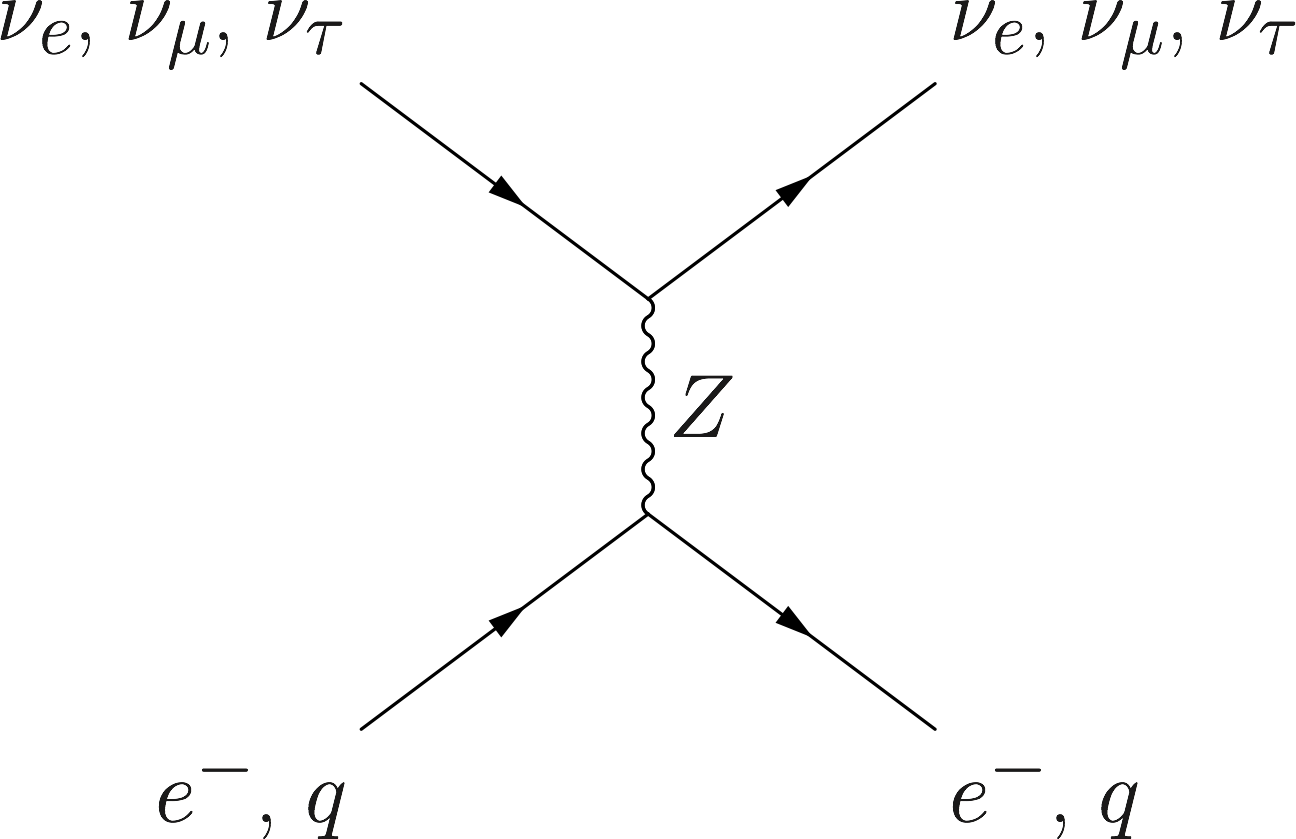
\includegraphics[scale=0.2]{Figures/Chapter1/neutral-current.png}
    \caption{Feynman diagram that shows the elastic scattering of a neutrino with electrons and nucleons. Figure taken from \cite{NCImage}.}
    \label{fig:NeutrinoInt:NC}
\end{figure}

For neutrino inelastic reactions, particularly those occurring at high energy, the production of pions can be observed. Examples include

\begin{equation}
    \begin{split}
        \nu_l + p \rightarrow \nu_l + p +\pi^0 \\
        \nu_l + p \rightarrow \nu_l + n +\pi^+ \\
        \nu_l + n \rightarrow \nu_l + n +\pi^0 \\
        \nu_l + n \rightarrow \nu_l + p +\pi^- \\
    \end{split}
\end{equation}

These kinds of interaction are also described by the W-S model. And for the cases where the neutrino interacts with the whole nucleus can be produced via coherent and incoherent interactions
\begin{equation}
    \begin{split}
        \nu_l + A \rightarrow \nu_l + A +\pi^0 \\
        \nu_l + A \rightarrow \nu_l + X +\pi^{\pm,0} \\
    \end{split}
\end{equation}

where $X$ corresponds to a nucleon. 

At higher energies the neutrino breaks up the nucleon producing a hadron shower; these interactions are known as NC Deep Inelastic Scattering (DIS). Some examples of the DIS interactions are: 

\begin{equation}
    \begin{split}
        \nu_l + (p,n) \rightarrow \nu_l + X \\
        \Bar{\nu}_l + (p,n) \rightarrow \Bar{\nu}_l + X \\
    \end{split}
\end{equation}

Here $X$ corresponds to a hadron jets. 

\subsection{Charged Current Neutrino interactions}
\label{Cap:Int:NuInteractions:CC}

In the Charged Current (CC) neutrino the neutrino interacts by the $W^\pm$ boson. The special interest around the CC interactions is that the neutrino change of identity produces a charged lepton, which can be detected and measured directly; in this way the incoming neutrino energy can be estimated. At the same time, the neutrino flavor can be identified. Therefore, this type of interaction is very important for neutrino oscillation experiments. A general Feynman diagram of a CC interaction is shown the \textbf{Figure} \ref{fig:Int:NuInteractions:CCFeynman}. 

\begin{figure}[!htb]
    \centering
    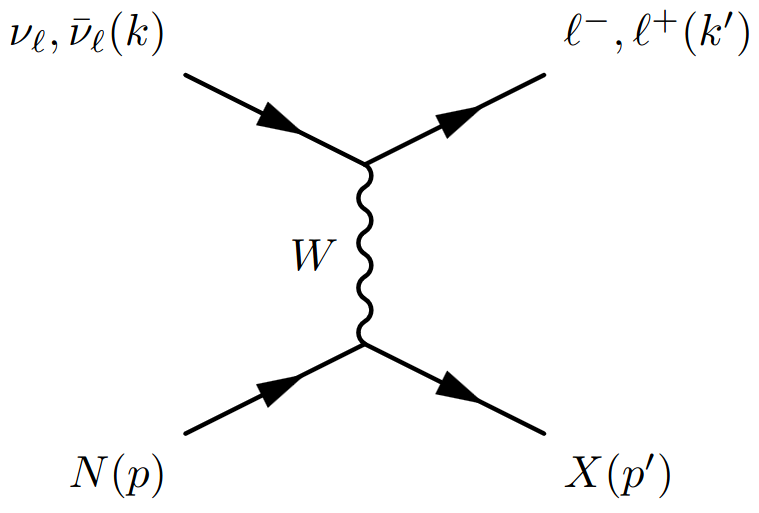
\includegraphics[scale=0.3]{Figures/Chapter1/CCFeynmanDiag.png}
    \caption{General CC neutrino interaction Feynman diagram. $N$ is a nucleon, and $X$ is the hadronic recoil system. Figure by the author.}
    \label{fig:Int:NuInteractions:CCFeynman}
\end{figure}

CC neutrino interactions can be categorized by invariant hadronic mass ($W$). The Feynman diagram of the \textbf{Figure} \ref{fig:Int:NuInteractions:CCFeynman} $W$ is defined as follows: 

\begin{equation}
    W^2 = p'^2 = (k +  p - k')^2
\end{equation}
 where $k$, $k'$, $p$ and $p'$ are the four momenta of the incident neutrino, the final state lepton, nucleon and the total four momenta of the hadronical recoil system. 

 The most common interactions produced by CC neutrino interactions as function of $W$ are 
 
\begin{itemize}
    \item \textbf{Quasi-elastic (QE)}: The reaction for the CCQE interactions is $\nu_\ell(\Bar{\nu}_\ell) + n(p)\rightarrow \ell^- (\ell^+) + p (n)$. These reactions occur around $W \approx m_N$, where $m_N$ is the mass of the nucleon. As depicted in the reaction, the nucleon changes to its isospin partner. An example of a Feynman diagram for the CCQE interaction is shown in Figure \ref{fig:Int:NuInteractions:CCQEFeynman}.

    \begin{figure}[!htb]
        \centering
        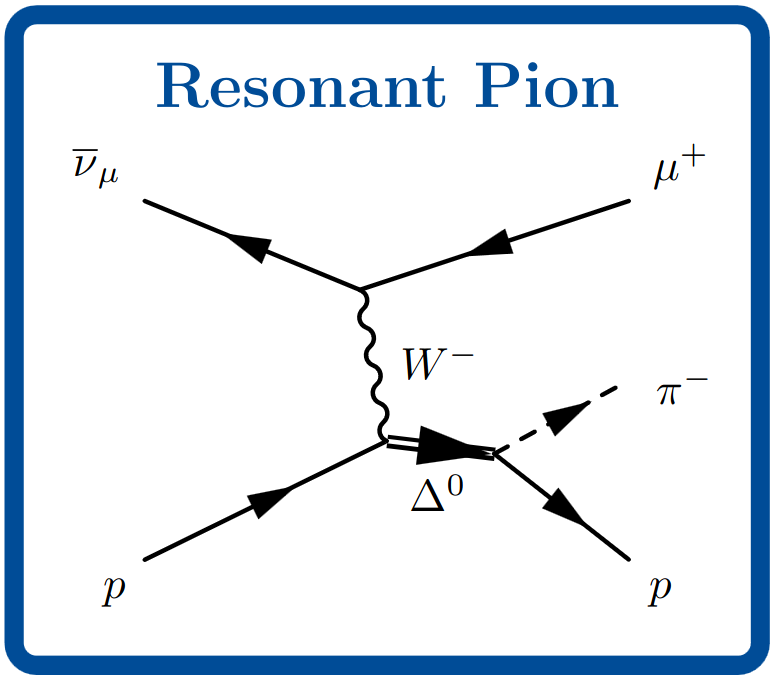
\includegraphics[scale=0.25]{Figures/Chapter1/ResonantChannel.png}
        \caption{Feynman diagram of the CC QE neutrino interaction. Figure by the author.}
        \label{fig:Int:NuInteractions:CCQEFeynman}
    \end{figure}
    
    \item \textbf{Resonant}: The general reaction that describes these interactions is $\nu_\ell(\Bar{\nu}_\ell) + N\rightarrow \ell^- (\ell^+) + N' + \pi$. These interactions produce a resonance baryon that decays rapidly and produces one charged or neutral pion before exiting the nucleus. They are produced in the $m_\Delta \lesssim W \lesssim 1.8$ GeV region.

    \begin{figure}[!htb]
        \centering
        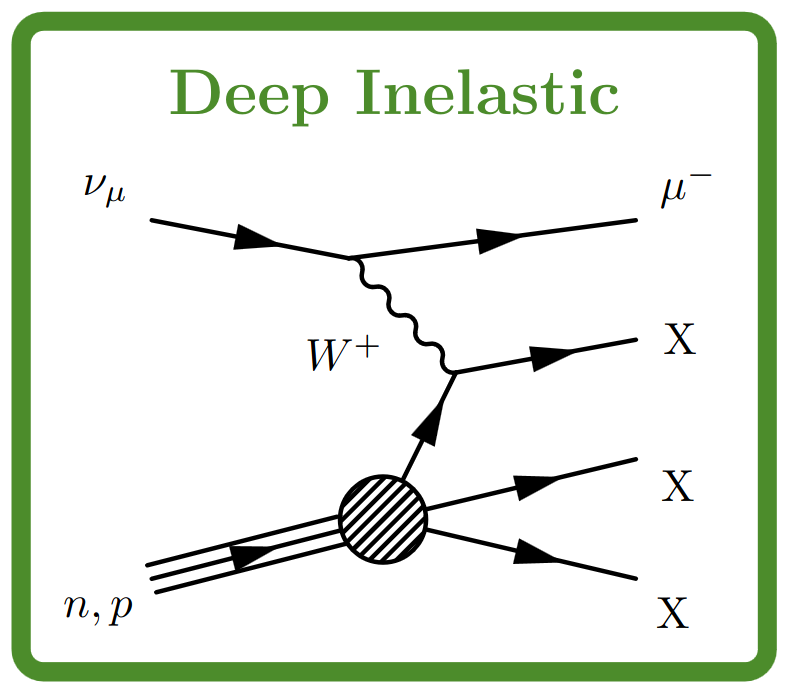
\includegraphics[scale=0.25]{Figures/Chapter1/DISChannel.png}
        \caption{Feynman diagram of the CC Resonant neutrino interaction. Figure by the author.}
        \label{fig:Int:NuInteractions:CCRESFeynman}
    \end{figure}
    
    \item \textbf{Deep Inelastic Scattering (DIS)}: The general reaction for the DIS interactions is $\nu_\ell(\Bar{\nu}_\ell) + n(p)\rightarrow \ell^- (\ell^+) + X$, where $X$ is a hadrons jet. In this interactions the neutrino interacts directly with the quarks breaking up the nucleus and producing an hadronic shower.

        \begin{figure}[!htb]
        \centering
        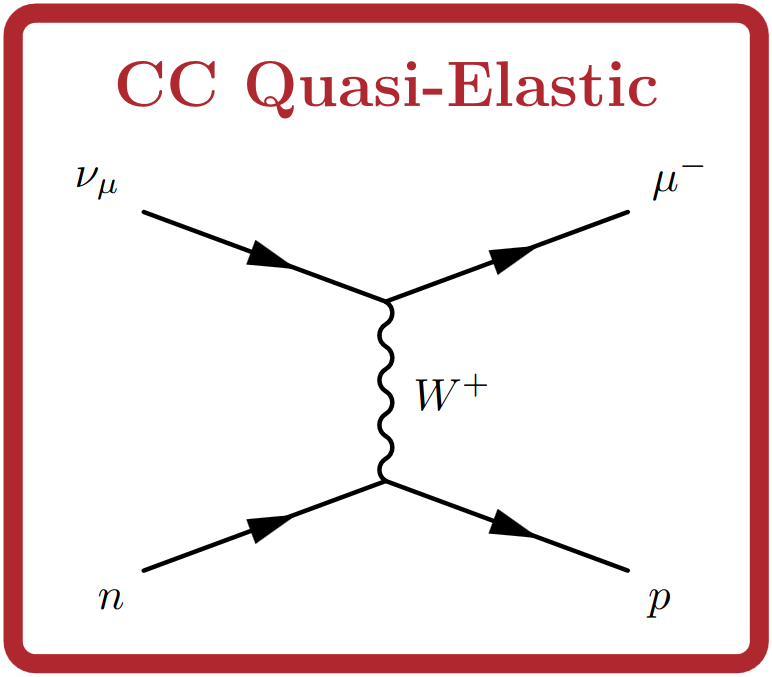
\includegraphics[scale=0.25]{Figures/Chapter1/CCQEChannel.png}
        \caption{Feynman diagram of the CC DIS neutrino interaction. Figure by the author.}
        \label{fig:Int:NuInteractions:CCDISFeynman}
    \end{figure}
\end{itemize}

\begin{figure}[!htb]
    \centering
    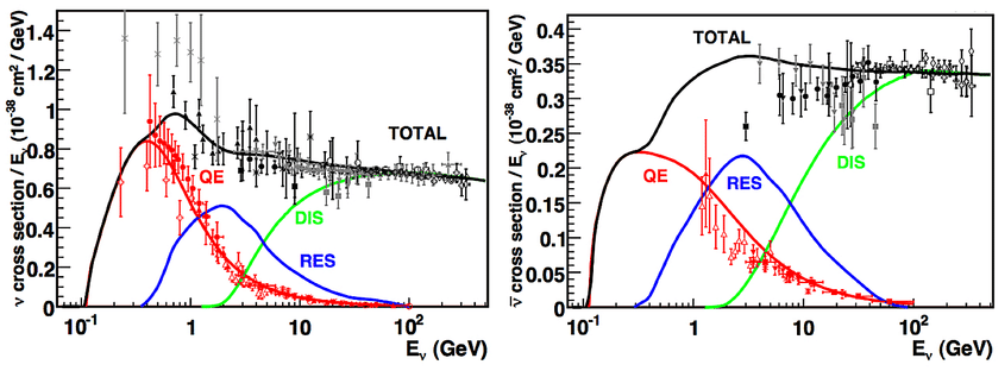
\includegraphics[scale=0.35]{Figures/Chapter1/InteractionChannels.png}
    \caption{The total cross section distributions for CC neutrino and antineutrino interaction as function of the neutrino energy is shown. The data points are provided by multiple experiments. It also shows the simulated CCQE, resonant and DIS cross section. Figure taken from \cite{Formaggio_2012}.}
    \label{fig:Int:NuInteractions:CCXSecChannels}
\end{figure}

In the \textbf{Figure} \ref{fig:Int:NuInteractions:CCXSecChannels} the cross section for the different neutrino interaction channels is shown. From the plots, it can be observed that for different neutrino energies there is a predominant interaction type. It is important to note that there are other CC interactions that are not included in those plots, such as coherent interactions and 2p2h interactions.  

\subsubsection{CC Quasi-elastic scattering model (CCQE)}
\label{Cap:Int:NuInteractions:CCQEmodel}
The differential cross section for the CCQE interactions is provided by the Llewellyn-Smith model \cite{LLEWELLYNSMITH1972261}. It is obtained as a function of the four-momentum transfer ($Q^2$) which is the negative value of the Mandelstam variable $t$: 

\begin{equation}
    \begin{split}
        Q^2 = -q^2 = -t = -(p_\nu - p_\ell)^2\\
        s = (p_\nu + p_N)^2 \\
        u = (p_\ell + p_N)^2
    \end{split}
\end{equation}
where $p_\nu$, $p_N$ and $p_\ell$ and are the four momentum of the neutrino, nucleon and lepton, respectively.

The model is described in terms of the form factors which attempt to describe the internal structure of a nucleon in a rest frame. 

\begin{equation}
    \frac{d\sigma}{dQ^2} = \frac{m^4_N G^2_F|V_{ud}|^2}{8\pi(p_\nu \cdot p_N)^2}\left(A(Q^2)\pm B(Q^2)\frac{s-u}{m^2_N}+C(Q^2)\frac{(s-u)^2}{m^4_N}\right)
\end{equation}

where $m_N$ is the mass of the nucleon, $G_F$ is the reduced Fermi constant ($1.166 \times 10^{−5}\ GeV^{−2}$), $V_{ud}$ is the CKM matrix describing the transition probability between the $u$ and $d$ quarks, $A$, $B$ and $C$ are functions of form factors. 

This model has two vector form factors $F^1_V (Q^2)$ (Dirac electromagnetic isovector form factor) and $F^2_V (Q^2)$ (Pauli electromagnetic isovector form factor), the axial form factor $F_A(Q^2)$ and the pseudoscalar form factor $F_P(Q^2)$. The vector form factor are obtained from the results of the electron-nucleon scattering experiments. This is due to the conservation of the vector current hypothesis for the electromagnetic and weak vector currents. 

In the case of $F_A$, it is also obtained from the electron scattering experiments at low $Q^2$ based on a dipole approximation in terms of the axial mass:

\begin{equation}
    F_A(Q^2) = \frac{g_A}{\left(1 + \frac{Q^2}{M^2_{A,CCQE}}\right)^2}
\end{equation}
where $g_A$ is the axial coupling constant, it is measured from the neutron lifetime. The $M_{A,CCQE}$ is the axial mass which is given from the CCQE neutrino cross section experiments.

The $F_P$ form factor can be related to $F_A$ scaled by a factor of $m^2_\ell / m^2_N$. The contribution of $F_P$ is small even if it is possible to just ignore this when the experiments do not have a good resolution to measure this parameter model.


\subsubsection{Resonant pion production model}
\label{Cap:Int:NuInteractions:RESmodel}

The neutrino interacts with the nucleon producing a baryon resonance. The baryon decays quickly, producing a nucleon and a pion. In oscillation experiments, usually the resonances with isospin 1/2 ($N*$) and with isospin 3/2 ($\Delta$) are produced. \textbf{Figure} \ref{fig:Int:NuInteractions:Resmodel:FaymanDiag} shows a general Feynman diagram of resonant interactions.

\begin{figure}[!htb]
    \centering
    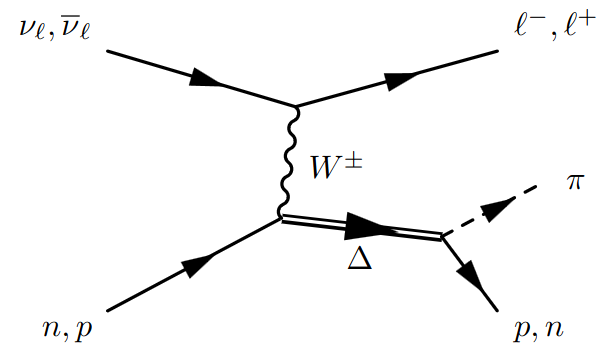
\includegraphics[scale=0.3]{Figures/Chapter1/ResonantInt.png}
    \caption{General Feynman diagram representing the resonant interactions. Figure by the author.}
    \label{fig:Int:NuInteractions:Resmodel:FaymanDiag}
\end{figure}

The Rein-Sehgal model \cite{REIN198179} predicts the resonant pion production by neutrino interactions. It 18 different resonances for $W<2$ GeV for 14 different reactions. The differential cross section with respect to $Q^2$ and $E_{had}$ defined for a sharp peak for a resonance width is given by:

\begin{equation}
    \frac{d^2\sigma}{dQ^2dE_{had}}=-\frac{G^2_F}{4\pi^2}\frac{Q^2}{|\Vec{p}|^2} k (u^2\sigma_L + \nu^2\sigma_R + 2u\nu\sigma_0)\delta(W-M_{res})
\end{equation}
where $|\Vec{p}|$ is the three momentum of the virtual boson, $M_{res}$ is the mass of the resonance, $m^2_N$ is the mass of the nucleon, $\sigma_L$/$\sigma_R$/$\sigma_0$ is the partial cross section of left/right/zero handed helicity, and $u$, $\nu$ and $k$ are defined as follow:
\begin{equation}
    \begin{split}
        k = \frac{M^2_{res}-m^2_N}{2m_N}\\
        u = \frac{E_nu + E_l + |\Vec{p}|}{2E_\nu}\\
        \nu = \frac{E_nu + E_l - |\Vec{p}|}{2E_\nu}
    \end{split}
\end{equation}

The $\delta$-function produces a sharp peak cross section, to produce a narrow width approximation the $\delta$-function can be replaced by a Breit-Wigner factor

\begin{equation}
    \delta(W-M_{res})\rightarrow\frac{1}{2\pi}\frac{\Gamma}{(W-M)^2+\Gamma^2/4}
\end{equation}
where $\Gamma$ is the width of the resonance.

The helicity cross sections $\sigma_{L,R,0}$ are 
\begin{equation}
    \begin{split}
        \sigma_{L,R}(Q^2) = \frac{\pi M_{res}}{2m_N k}\sum_{spins}|f_\mp|^2\\
        \sigma_{0}(Q^2) = \frac{\pi m_N }{2 M_{res} k}\left(\frac{|\Vec{p}|^2}{Q^2}\right)\sum_{spins}|f_0|^2
    \end{split}
\end{equation}
where $f_\mp$ and $f_0$ are the helicity amplitudes that are given by the relativistic quark model from Feynman, Kislinger, and Ravndal (FKR) \cite{PhysRevD.3.2706}. These amplitudes are functions of the axial ($G^A_{res}$) and vector ($G^V_{res}$) form factors modeled as dipoles:

\begin{equation}
    G^{A,V}_{res} (Q^2)= \left(1+ \frac{Q^2}{4M^2_N}\right)^{1/2-n}\left(\frac{1}{1+\frac{Q^2}{M^2_{A,V\ res}}} \right)^2
\end{equation}
where $n$ is the number of oscillator quanta observed in the resonance, $M_{A\ res} = 1.12$ GeV and $M_{V\ res} = 0.84$ GeV


\subsubsection{Deep Inelastic Scattering Interactions model (DIS)}
\label{Cap:Int:NuInteractions:DISmodel}

At higher energies, the neutrino interacts with quarks, breaking up the nucleons, generating jets of hadrons. In DIS scattering, the hadron parts (quarks and gluons) are modeled as free particles called \textit{partons}. Charged partons correspond to the quarks, and neutral partons that correspond to the gluons. To describe these systems, the following Lorentz invariants are defined, inelasticity \textit{y} and the Bjorken variable \textit{x}:

\begin{equation}
    \begin{split}
        x = \frac{Q^2}{2m_N v} \\
        y = \frac{v}{E_\nu}
    \end{split}
\end{equation}
where $v= E_{\nu_\ell} - E_\ell$. For the lab frame where the nucleon momentum is assumed to be zero, $v = E_{had}$.
The cross section for DIS scattering in terms of $x$ and $y$ is:

\begin{equation}
    \begin{split}
        \frac{d^2\sigma}{dxdy}= & \frac{G^2_F m_N E_\nu}{\pi}\left(1 + \frac{Q^2}{m^2_W}\right)^{-2} \dots\\
        & \dots \left[xy^2F^{W^\pm N}_1 + \left(1-y-\frac{xym_N}{2E_\nu} \right)F^{W^\pm N}_2 \pm  xy\left(1-\frac{y}{2}\right)F^{W^\pm N}_3  \right]
    \end{split}
\end{equation}
where $m_W$ is the mass of the $W$ boson, for neutrinos the positive value of $\pm$ and the negative value for the antineutrino is taken. $F^{W\pm N}_i$ are the nucleon structure functions that describe the interaction of $W^\pm$ with the nucleon $N$. The structure functions give the probability of finding a quark with a four-momentum $p_i = xp_N$, these probabilities are found by the experimental results. Immediately after the neutrino breaks the nucleon, the quarks produce new quarks from the vacuum, producing \textit{hadronization}, which usually produces the hadron shower. 
\subsubsection{Coherent Interactions model}
\label{Cap:Int:NuInteractions:Coherent}

The coherent interaction is produced when the neutrino interacts with the nucleus as a whole. This interaction represents around 1\% of the CC interactions. These interactions are characterized by producing a pion in the final state and do not modify the nucleus. The square of the four-momentum exchange for the nucleus ($|t|=(p_\nu-p_\ell-p_\pi)$) is small. The Rein-Sehgal model \cite{REINcoh198329} predicts coherent interactions assuming that $Q^2 \rightarrow 0$. The \textbf{Figure} \ref{fig:Int:NuInteractions:Coherent} shows the Feynman diagram for the coherent interactions.


\begin{figure}[!htb]
    \centering
    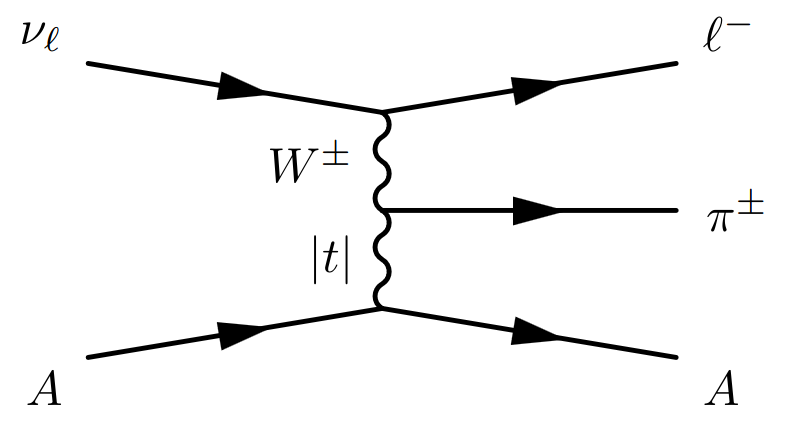
\includegraphics[scale=0.3]{Figures/Chapter1/CoherentFeynman.png}
    \caption{Feynman diagram for the coherent interaction. The $|t|$ corresponds to the four-momentum transferred to the nucleus. The nucleus $A$ does not change after the interaction. Figure by the author.}
    \label{fig:Int:NuInteractions:Coherent}
\end{figure}

\subsubsection{Diffractive Interactions model}
\label{Cap:Int:NuInteractions:Diffractive}

The diffractive interactions are similar to the coherent interactions, but the neutrino interacts with a proton instead of the nucleus. This type of interaction is produced specially by the interaction of the neutrino with hydrogen atoms. The diffractive interactions can also be described by the Rein-Sehgal model \cite{REINcoh198329}.

\begin{figure}[!htb]
    \centering
    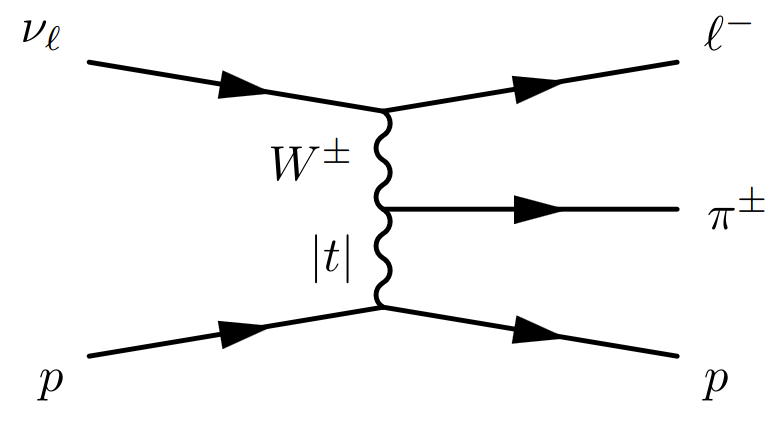
\includegraphics[scale=0.3]{Figures/Chapter1/DiffractiveFeynman.png}
    \caption{Feynman diagram for the diffractive interaction. $|t|$ corresponds to the four-momentum transferred to the proton. The $p$ does not change after the interaction. Figure by the author.} 
    \label{fig:Int:NuInteractions:Diffractive}
\end{figure}

\section{Final State Interactions (FSI)}
\label{Cap:Int:FSI}
To exit the nucleus, the products of neutrino interactions must pass through the nucleus. During their journey, they can interact with other particles within the nucleus, altering the kinematics of these particles or generating new ones. The particles emerging from the nucleus are referred to as Final State Interaction (FSI) particles. The interactions inside the nucleus smear the initial conditions of the neutrino interaction products; these effects make it difficult to measure the nature of the initial neutrino interaction. 

\begin{figure}[!htb]
    \centering
    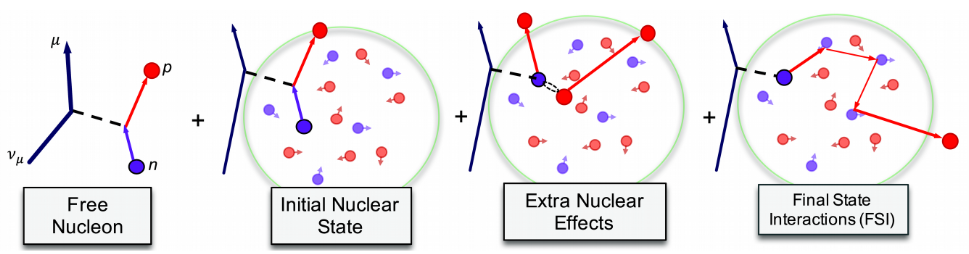
\includegraphics[scale=0.35]{Figures/Chapter1/FSIProcess.png}
    \caption{The resultant particles from the interaction can interact of different ways before to leave the nucleus. These nuclear effects are studied and simulated in the experiments. Figure taken from \cite{FSIFigure}.}
    \label{fig:Int:FSI:FSIProcess}
\end{figure}

The most significant effects of the nuclear effects are the following:

\begin{itemize}
    \item \textbf{Elastic Scattering:} These interactions just change the direction of the interaction product, but not the kinetic energy of it.  
    \item \textbf{Absorption:} The interaction products are absorbed by the nucleus, hence these do not leave the nucleus.
    \item \textbf{Inelastic Scattering:} In these interactions the products transfer part of their kinetic energy to the nucleons producing new particles that were not observed in the neutrino interaction vertex. 
    \item \textbf{Charge Exchange:} The charge of the interacting particle changes. For example the reaction $\pi^+ n \rightarrow \pi^0 p$.
\end{itemize}

The interactions inside the nucleus are difficult to model. The dynamics inside of the nucleus depends on the physics of many bodies; at the same time the strong interaction is present inside the nucleus. All of these interactions increase the difficulty of modeling FSI effects. FSI models are developed using data from external experiments.

To model the FSI effects using the data, the results from experiments in which pions or protons are scattered are used. In these experiments the initial conditions of the pions and protons are known, and the scatter gives information about how these interact with the components of different targets. However, this method does not exactly represent what is occurring in a neutrino interaction, where the pion or proton is produced inside the nucleus.

For the simulations, it uses the hadronic cascade simulation where the path of the resultant particles is divided into steps, and for each step the probability of the interaction with the nucleus is calculated by Monte Carlo methods. When the particle interacts with the nucleus, the four-momentum of the incident particle is randomly modified and depends on the kind of interaction or effect that is affecting the particle. The nuclear effect probabilities are estimated from experimental results or from theoretical models.

The pions are the lightest meson; therefore, these are commonly used to measure the effects of the nucleus on their kinematics. Some variables such as the Adler angles\cite{S_nchez_2016} can be used to study the nuclear effects because these are very sensitive to the nuclear effects.

\section{CC $\nu$ single pion production status}
\label{Cap:Int:Motivation}

Neutrino oscillation experiments are particularly interested in measuring CC neutrino interactions. This is because CC interactions not only reveal the incident neutrino flavor but also witness the neutrino's transformation into a charged lepton, facilitating direct energy reconstruction. Future and current neutrino oscillation experiments are designed to measure neutrinos with a few GeV to reduce the background produced by DIS where the energy reconstruction is more complicated due to the production of neutral particles and the theoretical models are more complicated. Therefore, it is easier to measure the neutrino interactions for a few GeV. For this energy region, there are multiple interactions that produce charged pions in the final state, such as resonant, non-resonant, coherent, or FSI.

 
\begin{figure}[!htb]
    \centering
    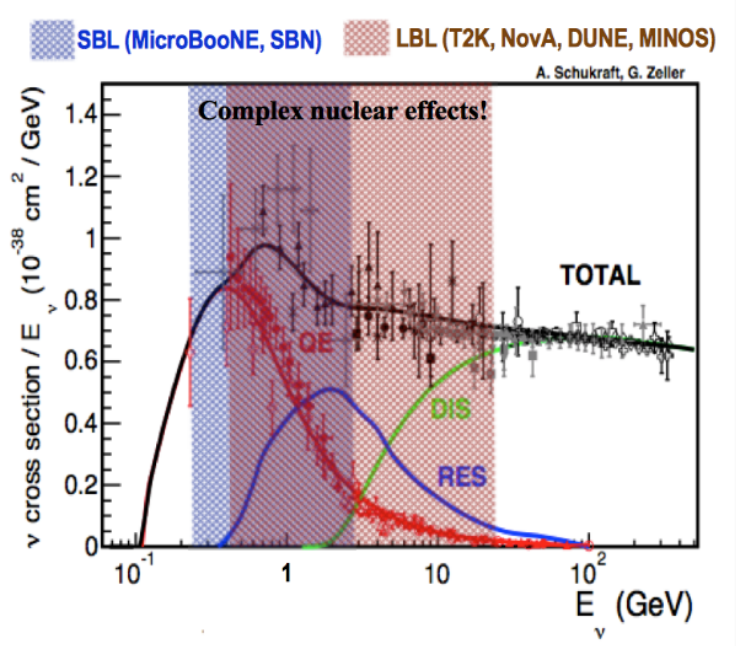
\includegraphics[scale=0.3]{Figures/Chapter1/nuXSec.png}
    \caption{neutrino cross section as function the neutrino energy. It shows the neutrino energy region where the current and future neutrino oscillation experiments take data. Figure taken from \cite{gollapinni2016neutrino}.}
    \label{fig:Int:Motivation:nuXsecl}
\end{figure}

The pions are also part of the background for the CCQE interactions. The most simple interaction that could be used to work in the oscillation experiments is the CCQE interactions; this is because the topology of this reaction is very simple and allows one to have a good reconstruction of the incident neutrino. However, nuclear effects and resonant and non-resonant interactions can fake QE interactions. The resonant and non-resonant interactions produce pions that can fake the proton and smear the neutrino energy reconstruction. At the same time, the study of the pion production is important in developing better nuclear models because these are more visible in the pion than in other particles. Therefore, it is crucial to study events in which the pions are produced. 

The initial experiments in which single-pion production is reported are the Argonne \cite{PhysRevD.25.1161} and Brookhaven \cite{PhysRevD.34.2554} National Laboratory bubble chamber experiments, which used hydrogen and deuterium, respectively, to measure neutrino interactions. The simplicity of the nuclear targets of these detectors reduces the nuclear effects and simplifies the interpretation of the data. A recent re-analysis increased the precision of these data\cite{PhysRevD.90.112017}.

Experiments such as T2K \cite{PhysRevD.95.012010}, MiniBooNE \cite{Aguilar_Arevalo_2011}, and MINER$\nu$A \cite{Eberly:2014mra, Bercellie.131.011801, PhysRevD.94.052005} have conducted measurements of pion production on various materials, including water, mineral oil, hydrocarbons, lead, iron, and carbon. Specifically, MINER$\nu$A obtained results for a neutrino beam energy peak at 3 GeV and another at 6 GeV.

The MINER$\nu$A experiment has reported results for the production of charged \cite{Bercellie.131.011801, Eberly:2014mra, PhysRevD.94.052005} and neutral \cite{PhysRevD.96.072003, Le_2015} pions in hydrocarbons (plastic scintillator) and other nuclear targets such as lead, water, iron and carbon. The design of this detector allows for measurements of neutrino interactions on various materials.

The most recent result of the $\nu_\mu CC1\pi^+$ channel \cite{Bercellie.131.011801} shows the measurement of pion production in different MINER$\nu$A regions for a neutrino energy peak of 6 GeV. The results also compare the cross sections with different event generators to assess the consistency with different models.

In both analyses, the results show disagreement between the data and the neutrino interaction generators, especially for the low $Q^2$ region. In addition, discrepancies between the data and the iron and lead models are observed in most variables. It suggests that better models are necessary for the production of pions in different materials. The systematic errors from the ME era show a strong dependency to the cross section and final state interaction models.  

The MINER$\nu$A results in LE and ME show results with an efficiency of $\sim$6\% and a purity of $\sim$ 68 \%, with a restriction for a low $T_\pi$ region given for the detector limitations to measure the pion track with a smaller energy of 35 MeV. However, the statistic error for the Medium Energy era is below the 5\% for most of the variables.  

The work developed in this thesis looks to improve the measurements for charged-pion production in hydrocarbons by implementing a technique that increases the data selection while increasing the kinematic phase space. It also shows the calculation of double differential cross section. 